\documentclass[12pt, a4paper]{article}

% ==========================================
% 1. KHAI BÁO GÓI THƯ VIỆN (PACKAGES)
% ==========================================
% Bảng mã & Font chữ
\usepackage[utf8]{inputenc}
\usepackage[T5]{fontenc}

% Toán học
\usepackage{amsmath, amssymb}

% Căn lề & Bố cục trang
\usepackage[top=2.2cm, bottom=1.5cm, left=1cm, right=1cm, headheight=15pt]{geometry}
\usepackage{fancyhdr}
\usepackage{needspace}
\usepackage{tkz-tab}

% Đồ họa & Màu sắc
\usepackage{xcolor}
\usepackage{graphicx} 
\usepackage{tikz}
\usetikzlibrary{calc, shapes.geometric, positioning}


% Bảng biểu & Danh sách
\usepackage{colortbl}
\usepackage{array}
\usepackage{makecell}
\usepackage{multirow}
\usepackage{tasks}

% Biểu tượng
\usepackage{fontawesome5}

% ==========================================
% 2. THIẾT LẬP MÀU SẮC CHỦ ĐẠO
% ==========================================
\definecolor{goldyellow}{RGB}{255, 179, 0}
\definecolor{amberorange}{RGB}{230, 115, 0}
\definecolor{lightamber}{RGB}{255, 248, 225}
\definecolor{deepblue}{RGB}{25, 42, 86}
\definecolor{accentred}{RGB}{232, 65, 24}
\definecolor{softgray}{RGB}{220, 220, 222} 
\definecolor{fbblue}{RGB}{15, 80, 200}


% ==========================================
% 3. CẤU HÌNH HEADER & FOOTER
% ==========================================
\pagestyle{fancy}
\fancyhf{}
\renewcommand{\headrulewidth}{0pt}

% Khai báo biến lưu trữ nội dung góc phải của Header
\newcommand{\HeaderRightText}{}

% --- Header ---
\fancyhead[C]{
    \begin{tikzpicture}[remember picture, overlay]
        
        % Dải màu trang trí góc trên
        \path[fill=deepblue] (current page.north west) -- (current page.north east) 
            -- ($(current page.north east) + (0, -1.6cm)$) 
            .. controls ($(current page.north) + (3, -2.0cm)$) and ($(current page.north) + (-3, -0.4cm)$) .. 
            ($(current page.north west) + (0, -1.0cm)$) -- cycle;
            
        \path[fill=goldyellow] (current page.north west) -- (current page.north east) 
            -- ($(current page.north east) + (0, -1.0cm)$) 
            .. controls ($(current page.north) + (4, -1.0cm)$) and ($(current page.north) + (-2, -2.2cm)$) .. 
            ($(current page.north west) + (0, -1.6cm)$) -- cycle;
            
        \path[fill=amberorange] (current page.north west) -- ($(current page.north west) + (6.5cm, 0)$) 
            .. controls ($(current page.north west) + (4.5cm, -1.2cm)$) and ($(current page.north west) + (2cm, -2.0cm)$) .. 
            ($(current page.north west) + (0, -2.0cm)$) -- cycle;
            
        % Logo góc trái Header
        \node[anchor=west, inner sep=0pt] 
            at ($(current page.north west) + (0cm, -0.8cm)$) {
\includegraphics[height=2.0cm]{../../../image/logo-header.png}};
            
        % Text góc phải Header (Tự động lấy từ đối số thứ 3 của \titlebox)
        \node[anchor=east, text=white, font=\small\bfseries\sffamily] 
            at ($(current page.north east) + (-0.8cm, -0.5cm)$) {\HeaderRightText};
    \end{tikzpicture}
}

% --- Footer ---
\fancyfoot[C]{
    \begin{tikzpicture}[remember picture, overlay]
        % Đường kẻ ngang
        \draw[amberorange, line width=1.5pt] 
            ($(current page.south west) + (0cm, 0.4cm)$) -- ($(current page.south east) + (0cm, 0.4cm)$);

        % Dải cong góc phải
        \path[fill=goldyellow] (current page.south east) -- ($(current page.south east) + (-5cm, 0)$) 
            .. controls ($(current page.south east) + (-3cm, 0.8cm)$) and ($(current page.south east) + (-1.5cm, 1.2cm)$) .. 
            ($(current page.south east) + (0, 1.2cm)$) -- cycle;

        % Mạng xã hội
        \node[anchor=west, inner sep=0pt] at ($(current page.south west) + (1cm, 0.8cm)$) {
            \small\sffamily
            \textcolor{fbblue}{\faFacebook\hskip 4pt Toán Anh Huy MATH-STER}
            \hskip 18pt
            \textcolor{black}{\faTiktok\hskip 4pt huymathster}
        };

        % Số trang
        \node[circle, fill=white, draw=amberorange, line width=1.5pt, text=deepblue, font=\large\bfseries\sffamily, inner sep=4pt, minimum size=0.8cm] 
            at ($(current page.south east) + (-1.2cm, 0.6cm)$) {\thepage};
    \end{tikzpicture}
}

% ==========================================
% 4. ĐỊNH NGHĨA MACRO: KHUNG TIÊU ĐỀ
% ==========================================
\newcommand{\titlebox}[3]{
    % Gán nội dung đối số #3 vào biến HeaderRightText
    \gdef\HeaderRightText{#3}
    
    \begin{center}
    \vspace*{-0.5cm}
    \begin{tikzpicture}
        % Khung vô hình (Phantom Box) định chuẩn kích thước
        \node[text width=16cm, inner xsep=0pt, inner ysep=16pt, opacity=0] (MainBox) {
            \begin{minipage}[c]{4.2cm}
                \centering\vspace{0.1cm}
                \rule{2.2cm}{2.2cm} 
                \vspace{0.1cm}
            \end{minipage}%
            \begin{minipage}[c]{11.5cm}
                \centering\vspace{0.15cm}
                {\huge\bfseries\sffamily #2 \par}
                \vspace{0.15cm} 
            \end{minipage}
        };
        
        % Đổ bóng & Nền
        \fill[goldyellow, rounded corners=8pt] ([xshift=5pt, yshift=-5pt]MainBox.south west) rectangle ([xshift=5pt, yshift=-5pt]MainBox.north east);
        \fill[white, rounded corners=8pt] (MainBox.south west) rectangle (MainBox.north east);
        
        % Lưới ô ly & Nền Logo
        \begin{scope}
            \clip[rounded corners=8pt] (MainBox.south west) rectangle (MainBox.north east);
            \draw[step=0.4cm, softgray!50, line width=0.6pt] (MainBox.south west) grid (MainBox.north east);
            \fill[lightamber!60] (MainBox.south west) rectangle ([xshift=4.2cm]MainBox.north west);
        \end{scope}

        % Viền ngoài
        \draw[deepblue, line width=1.5pt, rounded corners=8pt] (MainBox.south west) rectangle (MainBox.north east);

        % Nội dung Text (Lớp trên cùng)
        \node[text width=16cm, inner xsep=0pt, inner ysep=16pt] at (MainBox.center) {
            \begin{minipage}[c]{4.2cm}
                \centering
                % --- ĐIỀU CHỈNH TỌA ĐỘ LOGO Ở ĐÂY ---
                \hspace*{-0.5cm}\raisebox{-0.2cm}{
\includegraphics[width=5.5cm]{../../../image/logo.png}}
            \end{minipage}%
            \begin{minipage}[c]{11.5cm}
                \centering\vspace{0.15cm}
                {\huge\bfseries\sffamily\color{deepblue} #2 \par}
                \vspace{0.15cm} 
            \end{minipage}
        };
        
        % Trang trí phụ kiện
        \draw[deepblue, line width=1.5pt, dashed] ([xshift=4.2cm]MainBox.north west) -- ([xshift=4.2cm]MainBox.south west);
        \node[regular polygon, regular polygon sides=4, rotate=45, fill=white, draw=accentred, line width=1.2pt, inner sep=2.5pt] at ([xshift=4.2cm]MainBox.west) {};
        \node[anchor=west, fill=amberorange, text=white, font=\large\bfseries\sffamily, rounded corners=4pt, draw=deepblue, line width=1.5pt, inner xsep=12pt, inner ysep=6pt] at ([xshift=1.5cm]MainBox.north west) {#1};
        \fill[accentred] ([xshift=-1.8cm, yshift=-0.4cm]MainBox.north east) circle (3pt);
        \fill[amberorange] ([xshift=-1.4cm, yshift=-0.4cm]MainBox.north east) circle (3pt);
        \fill[goldyellow] ([xshift=-1.0cm, yshift=-0.4cm]MainBox.north east) circle (3pt);
    \end{tikzpicture}
    \vspace*{0cm}
    \end{center}
}

% ==========================================
% 5. ĐỊNH NGHĨA MACRO: CẤU TRÚC CÂU HỎI (ÉP SÁT NHAU)
% ==========================================
\newcommand{\questioncore}[2]{
    % Xóa khoảng cách phía trên, ép sát câu trước
    \noindent \textbf{\textcolor{deepblue}{Câu #1.} \textcolor{accentred}{[STER]}} #2
    \par\nopagebreak
}

% Cấu hình hiển thị đáp án trắc nghiệm
\settasks{
    label=\textbf{\textcolor{amberorange}{\Alph*.}}, 
    label-width=15pt,     
    item-indent=25pt,     
    label-offset=6pt,    
    column-sep=20pt,     
    after-item-skip=2pt  % Đã giảm tối đa khoảng cách giữa các dòng đáp án A B C D
}

% Hàm vẽ dòng kẻ nháp
\newcommand{\drawdashlines}[1]{
    \ifnum#1>0
        \nopagebreak\vspace{0.1cm}\noindent 
        \begin{tikzpicture}
            \foreach \i in {1,...,#1} {
                \draw[softgray, line width=0.2pt] (0,-{\i*0.75}) -- (\textwidth-4pt,-{\i*0.75});
            }
        \end{tikzpicture}
        \par
    \fi
    % Đã xóa hoàn toàn khoảng cách thừa ở nhánh else
}

% --- Dạng 1: Trắc nghiệm 4 đáp án ---
\newcommand{\questionLinesManual}[4]{
    \pgfmathsetmacro{\calculatedSpace}{1.5 + #1 * 0.65}
    \needspace{\calculatedSpace cm} 
    \questioncore{#2}{#3}
    #4
    \par\nopagebreak
    \drawdashlines{#1}
}

% --- Dạng 2: Trắc nghiệm Đúng/Sai ---
\newcommand{\questionTrueFalse}[4]{
    \pgfmathsetmacro{\calculatedSpace}{3.0 + #1 * 0.65} 
    \needspace{\calculatedSpace cm}
    \questioncore{#2}{#3}
    
    \nopagebreak
    \begin{center}
    \renewcommand{\arraystretch}{1.2} % Bóp nhỏ chiều cao của bảng Đ/S
    \begin{tabular}{|>{\centering\arraybackslash}m{0.8cm}|m{12cm}|>{\centering\arraybackslash}m{2cm}|>{\centering\arraybackslash}m{2cm}|}
        \hline
        \rowcolor{amberorange!20}
        & \multicolumn{1}{>{\centering\arraybackslash}m{12cm}|}{\textbf{\textcolor{deepblue}{Mệnh đề}}} & 
        \textbf{\textcolor{deepblue}{Đúng}} & 
        \textbf{\textcolor{deepblue}{Sai}} \\
        \hline
        #4
        \hline
    \end{tabular}
    \renewcommand{\arraystretch}{1}
    \end{center}
    
    \par\nopagebreak
    \drawdashlines{#1}
}

% ----- Dạng 3: Tự luận ngắn -----
\newcommand{\questionShortAnswer}[3]{
    \pgfmathsetmacro{\calculatedSpace}{1.5 + #1 * 0.8}
    \needspace{\calculatedSpace cm}
    
    {\linespread{1.1}\selectfont % Bóp nhỏ giãn dòng của câu tự luận
    \questioncore{#2}{#3}\par}
    
    \nopagebreak
    \begin{flushright}
        \begin{tikzpicture}
            \node[anchor=east, font=\small\bfseries\sffamily, text=deepblue] 
                at (-0.2, 0.4) {Đáp án:};
            \fill[goldyellow, rounded corners=3pt] (0.08, -0.08) rectangle (3.08, 0.72);
            \draw[draw=deepblue, fill=white, line width=1.2pt, rounded corners=3pt] 
                (0,0) rectangle (3.0, 0.8);
            \foreach \x in {0.75, 1.5, 2.25} {
                \draw[draw=deepblue, line width=0.6pt] (\x, 0) -- (\x, 0.8);
            }
        \end{tikzpicture}
    \end{flushright}
    
    \par\nopagebreak
    \drawdashlines{#1}
}

% ==========================================
% BẮT ĐẦU NỘI DUNG TÀI LIỆU
% ==========================================
\begin{document}

% Truyền 3 tham số: {Nhãn cam} {Chữ to chính giữa} {Chữ ở góc phải Header}
\titlebox{Chủ đề: Hàm số}{Kiểm tra cực trị của hàm số}{Hàm số: Cực trị}

\questionLinesManual{0}{1}{Cho hàm số \( f(x) \) có bảng biến thiên như sau:
\begin{center}
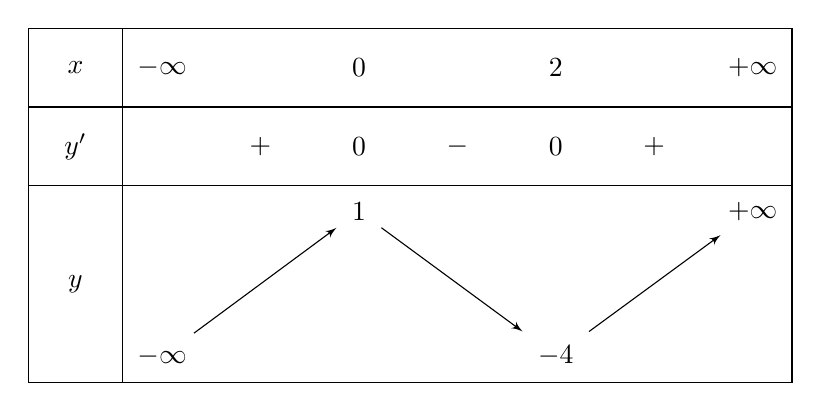
\begin{tikzpicture}[>=stealth]
    \tkzTabInit[nocadre=false,lgt=1.2,espcl=2.5]
    {$x$ / 1, $y'$ / 1, $y$ / 2.5}
    {$-\infty$, $0$, $2$, $+\infty$}
    \tkzTabLine{ , +, 0, -, 0, + }
    \tkzTabVar{-/$-\infty$, +/$1$, -/$-4$, +/$+\infty$}

\end{tikzpicture}
\end{center}
Hàm số đã cho đạt cực tiểu tại điểm nào sau đây?}{%
\begin{tasks}(4)
\task \( x = -4 \)
\task \( x = 2 \)
\task \( x = 1 \)
\task \( x = 0 \)
\end{tasks}
}

% ====== CÂU 3 ======
\questionLinesManual{0}{2}{Cho hàm số \( y = f(x) \) có bảng biến thiên sau:
\begin{center}
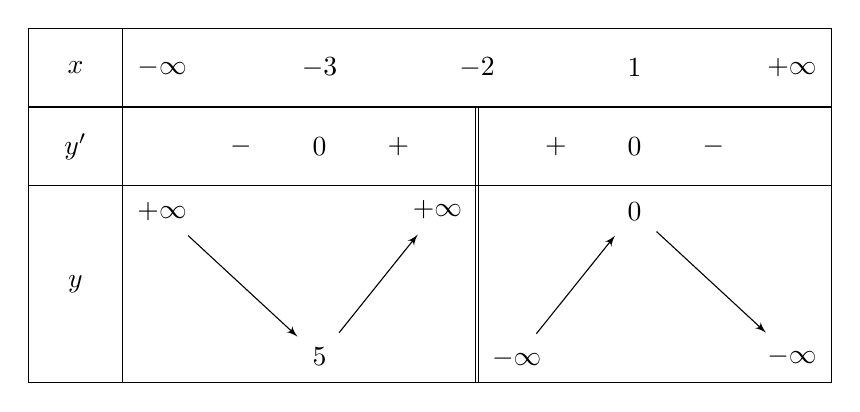
\begin{tikzpicture}[>=stealth]
    \tkzTabInit[nocadre=false,lgt=1.2,espcl=2]
    {$x$ / 1, $y'$ / 1, $y$ / 2.5}
    {$-\infty$, $-3$, $-2$, $1$, $+\infty$}
    \tkzTabLine{ , -, 0, +, d, +, 0, - }
    \tkzTabVar{+/$+\infty$, -/$5$,+D-/$+\infty$ /$-\infty$, +/$0$, -/$-\infty$}

\end{tikzpicture}
\end{center}
Giá trị cực đại của hàm số \( y = f(x) \) là:}{%
\begin{tasks}(4)
\task 0
\task 1
\task $-3$
\task 5
\end{tasks}
}

\questionLinesManual{0}{3}{Cho hàm số \( f(x) \) có bảng biến thiên như sau:
\begin{center}
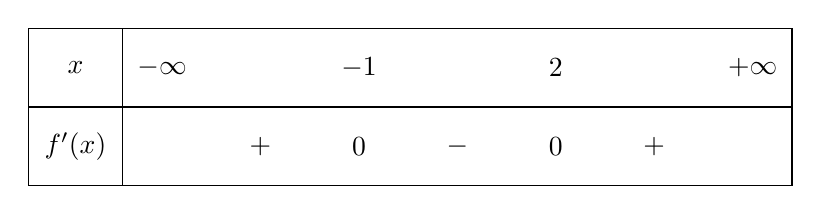
\begin{tikzpicture}[>=stealth]
    \tkzTabInit[nocadre=false,lgt=1.2,espcl=2.5]
    {$x$ / 1, $f'(x)$ / 1}
    {$-\infty$, $-1$, $2$, $+\infty$}
    \tkzTabLine{ , +, 0, -, 0, + }
\end{tikzpicture}
\end{center}
Hàm số đã cho đạt cực đại tại}{%
\begin{tasks}(4)
\task \( x = -2 \)
\task \( x = 2 \)
\task \( x = 1 \)
\task \( x = -1 \)
\end{tasks}
}

\questionLinesManual{0}{4}{Cho hàm số \( y = f(x) \) xác định trên \(\mathbb{R} \setminus \{1\}\) có bảng xét dấu như sau:
\begin{center}
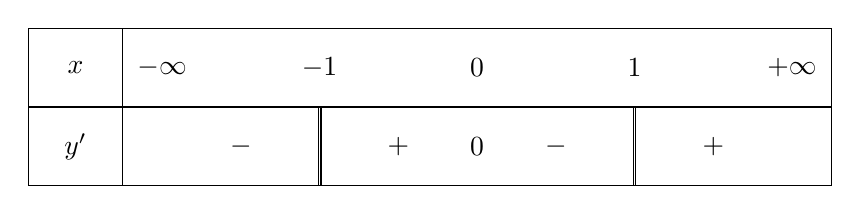
\begin{tikzpicture}[>=stealth]
    \tkzTabInit[nocadre=false,lgt=1.2,espcl=2]
    {$x$ / 1, $y'$ / 1}
    {$-\infty$, $-1$, $0$, $1$, $+\infty$}
    \tkzTabLine{ , -, d, +, 0, -, d, + }
\end{tikzpicture}
\end{center}
Hàm số có bao nhiêu điểm cực trị}{%
\begin{tasks}(4)
\task 0
\task 1
\task 2
\task 3
\end{tasks}
}

\questionLinesManual{0}{5}{Cho hàm số \( y = ax^3 + bx^2 + cx + d \) (\( a, b, c, d \in \mathbb{R} \)) có đồ thị như hình vẽ bên. Số điểm cực trị của hàm số này là
\begin{center}
\begin{tikzpicture}[>=latex, scale=0.8]
    % Hệ trục tọa độ
    \draw[->] (-3.5,0) -- (3.5,0) node[below] {$x$};
    \draw[->] (0,-3.5) -- (0,3.5) node[right] {$y$};
    \node[above left] at (0,0) {$O$};
    
    
    % Vẽ đồ thị hàm bậc 3 y = x^3 - 3x
    \draw[thick, color=black!80, samples=150, domain=-2.1:2.1] 
        plot (\x, {\x*\x*\x - 3*\x});
    
\end{tikzpicture}
\end{center}}{%
\begin{tasks}(4)
\task 3
\task 2
\task 0
\task 1
\end{tasks}
}

\questionLinesManual{0}{6}{Cho hàm số \( y = f(x) \) có đồ thị như hình vẽ
\begin{center}
\begin{tikzpicture}[>=latex, scale=0.8]
    % Hệ trục tọa độ
    \draw[->] (-3.5,0) -- (3.5,0) node[below] {$x$};
    \draw[->] (0,-3.5) -- (0,3.5) node[right] {$y$};
    \node[above left] at (0,0) {$O$};
    
    % Đánh dấu các điểm trên trục
    \node[below] at (-1,0) {$-1$};
    \node[below] at (1,0) {$1$};
    \node[right] at (0,-2) {$-2$};
    \node[left] at (0,2) {$2$};
    
    % Vẽ đồ thị hàm số bậc 3 y = x^3 - 3x
    \draw[thick, color=black!80, samples=150, domain=-3:-0.3] 
       plot (\x, {(\x*\x + 1)/\x});
    \draw[thick, color=black!80, samples=150, domain=0.3:3] 
       plot (\x, {(\x*\x + 1)/\x});
    % Đường nét đứt
    \draw[dashed] (-1,0) -- (-1,-2) -- (0,-2);
    \draw[dashed] (1,0) -- (1,2)-- (0,2);
\end{tikzpicture}
\end{center}
Giá trị cực tiểu của hàm số đã cho là}{%
\begin{tasks}(4)
\task 1
\task $-1$
\task $-2$
\task 2
\end{tasks}
}

\questionLinesManual{0}{7}{Cho hàm số \( y = x^3 - 3x^2 + 2 \). Mệnh đề nào dưới đây đúng?}{%
\begin{tasks}(2)
\task Hàm số đạt cực tiểu tại điểm \( x = 0 \)
\task Hàm số đạt cực đại tại điểm \( M(0; 2) \)
\task Hàm số đạt cực đại tại điểm \( x = 0 \)
\task Hàm số đạt cực đại tại điểm \( x = 2 \)
\end{tasks}
}

\questionLinesManual{0}{8}{Hàm số \( y = \dfrac{2x + 3}{x + 1} \) có bao nhiêu điểm cực trị?}{%
\begin{tasks}(4)
\task 1
\task 3
\task 0
\task 2
\end{tasks}
}

\questionLinesManual{0}{9}{Cho hàm số \( f(x) \) có đạo hàm \( f'(x) = x^3(x-1)(x-2) \), \( \forall x \in \mathbb{R} \). Số điểm cực trị của hàm số đã cho là}{%
\begin{tasks}(4)
\task 1
\task 3
\task 5
\task 2
\end{tasks}
}

\questionLinesManual{0}{10}{Cho hàm số \( y = f(x) \) có đạo hàm trên \( \mathbb{R} \). Biết hàm số \( y = f'(x) \) có đồ thị như hình vẽ. Phát biểu nào sau đây là đúng?
\begin{center}
\begin{tikzpicture}[>=latex, scale=0.8]
    % Hệ trục tọa độ
    \draw[->] (-3.5,0) -- (3.5,0) node[below] {$x$};
    \draw[->] (0,-2) -- (0,3.5) node[right] {$y$};
    \node[above left] at (0,0) {$O$};
    
    % Đánh dấu các điểm
    \node[below] at (-2,0) {$-2$};
    \node[below] at (1,0) {$1$};
    \node[right] at (0,2) {$2$};
    
    % Vẽ đồ thị f'(x) là parabol hướng xuống có nghiệm tại x = -2 và x = 1
    \draw[thick, color=black!80, samples=150, domain=-2.3:1.3] 
        plot (\x, {-(\x+2)*(\x-1)});
    
    \node[right] at (1.5,2) {$y = f'(x)$};
\end{tikzpicture}
\end{center}}{%
\begin{tasks}(1)
\task Hàm số \( y = f(x) \) đạt cực đại tại \( x_1 = -2 \) và đạt cực tiểu tại \( x_2 = 1 \).
\task Hàm số \( y = f(x) \) đạt cực tiểu tại hai điểm \( x_1 = -2 \) và \( x_2 = 1 \).
\task Hàm số \( y = f(x) \) đạt cực đại tại hai điểm \( x_1 = -2 \) và \( x_2 = 1 \).
\task Hàm số \( y = f(x) \) đạt cực tiểu tại \( x_1 = -2 \) và đạt cực đại tại \( x_2 = 1 \).
\end{tasks}
}

\end{document}